\documentclass[11pt,psfig]{article}
\usepackage{epsfig}
\usepackage{times}
\usepackage{amssymb}
\usepackage{float}

\newcount\refno\refno=1
\def\ref{\the\refno \global\advance\refno by 1}
\def\ux{\underline{x}}
\def\ut{\underline{\theta}}
\def\umu{\underline{\mu}}
\def\be{p_e^*}
\newcount\eqnumber\eqnumber=1
\def\eq{\the \eqnumber \global\advance\eqnumber by 1}
\def\eqs{\eq}
\def\eqn{\eqno(\eq)}

 \pagestyle{empty}
\def\baselinestretch{1.1}
\topmargin1in \headsep0.3in
\topmargin0in \oddsidemargin0in \textwidth6.5in \textheight8.5in
\begin{document}
\setlength{\parskip}{1.2ex plus0.3ex minus 0.3ex}


\thispagestyle{empty} \pagestyle{myheadings} \markright{Homework
5: CS 274A, Probabilistic Learning: Winter 2014}



\title{CS 274A Homework 5}
\author{Zachary DeStefano, 15247592}
\date{Due Date: Wednesday March 5th}

\maketitle

 \newpage

\section{Results for Dataset1}

\subsection{k-Means Plots}

\begin{figure}[H]
\centering
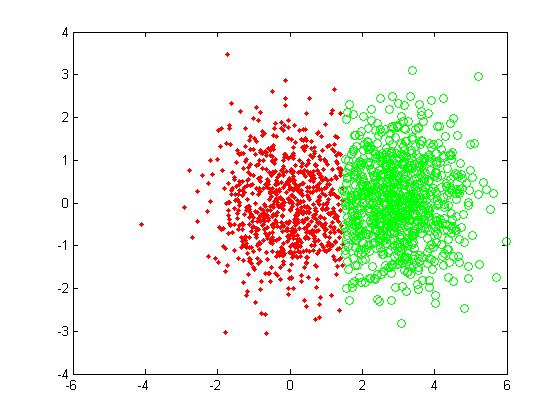
\includegraphics[height=3.25in]{dataset1_kMeansPlot.jpg}
\caption{The k-Means plot for dataset1, K=2}
\end{figure}

\begin{figure}[H]
\centering
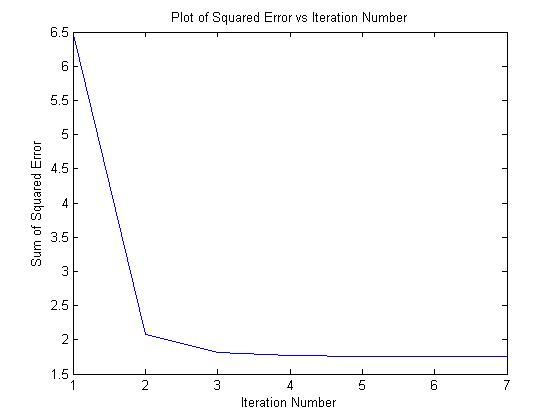
\includegraphics[height=3.25in]{dataset1_kMeans_squaredErrorPlot.jpg}
\caption{The Sum of Squared Error plot for dataset1, K=2}
\end{figure}

\subsection{EM Plots}

\begin{figure}[H]
\centering
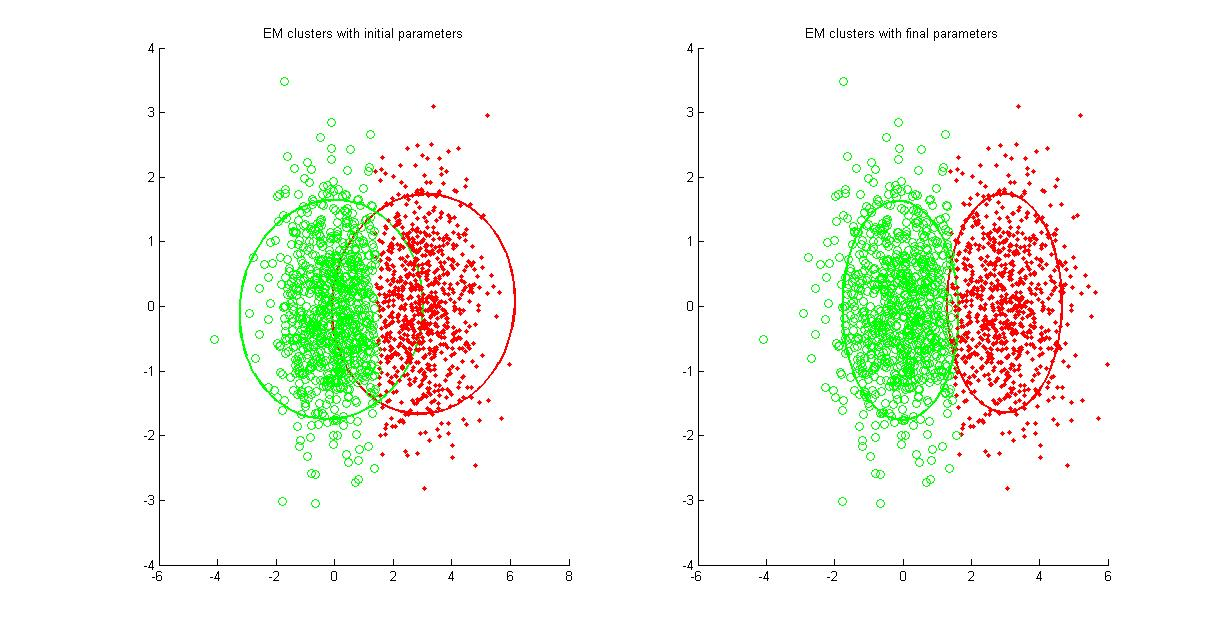
\includegraphics[height=3.25in]{dataset1_EMclusterPlots.jpg}
\caption{The EM cluster plots for dataset1, K=2, using initialization method 3}
\end{figure}

\begin{figure}[H]
\centering
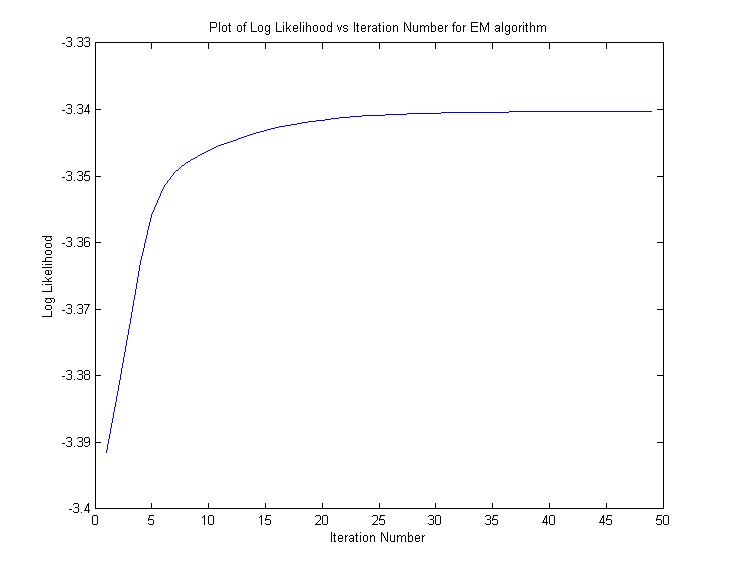
\includegraphics[height=3.25in]{dataset1_EMlogLikelihoodPlot.jpg}
\caption{The likelihood plot for dataset1, K=2, using initialization method 3}
\end{figure}

\subsection{Comments on k-Means and EM Results}

For dataset1, there was not much of a difference between the k-Means result and the EM algorithm result. This was likely due to the fact that the two Gaussians did not overlap so k-Means put the points in the correct cluster easily. When I computed the best initialization method, k-Means proved to be the best one for this data set. This makes sense because the data was easily able to be grouped into two sets using k-Means. 

\subsection{Comments on BIC test results}

\begin{table}[H]
  \centering
  \begin{tabular}{|c|c|c|}
    \hline
    \multicolumn{3}{|c|}{Dataset 1} \\\hline
    K & log likelihood & BIC value \\\hline
    1 & -5459.40 & -5481.53 \\
		2 & -5344.47 & -5388.73 \\
		3 & -5343.42 & -5409.82 \\
		4 & -5341.18 & -5429.72 \\
    5 & -5337.96 & -5448.63 \\\hline
  \end{tabular}
\end{table}

For dataset1, as expected, the log likelihood increases when you increase K, the number of clusters. When you use BIC to get the ideal number of clusters, we find that the BIC value is maximized at K=2. This is the solution we want since the data should be grouped into 2 clusters. 

\section{Plots for Dataset2}

\subsection{k-Means Plots}

\begin{figure}[H]
\centering
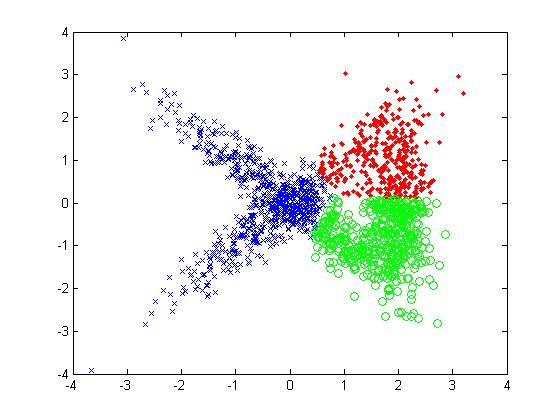
\includegraphics[height=3.25in]{dataset2_kMeansPlot.jpg}
\caption{The k-Means plot for dataset2, K=3}
\end{figure}

\begin{figure}[H]
\centering
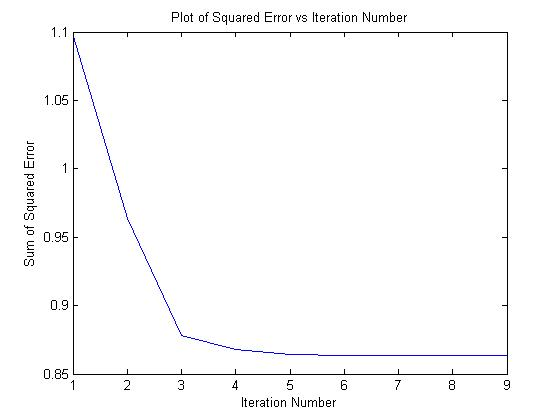
\includegraphics[height=3.25in]{dataset2_kMeans_squaredErrorPlot.jpg}
\caption{The Sum of Squared Error plot for dataset2, K=3}
\end{figure}

\subsection{EM Plots}

\begin{figure}[H]
\centering
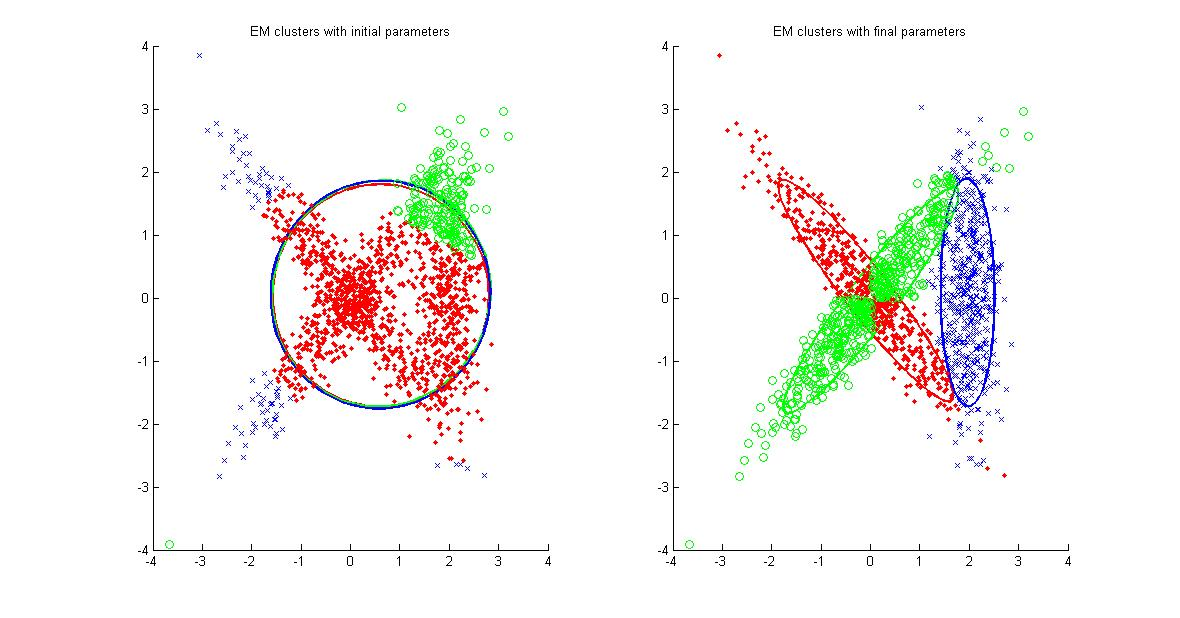
\includegraphics[height=3.25in]{dataset2_EMclusterPlots.jpg}
\caption{The EM cluster plots for dataset2, K=3, using initialization method 1}
\end{figure}

\begin{figure}[H]
\centering
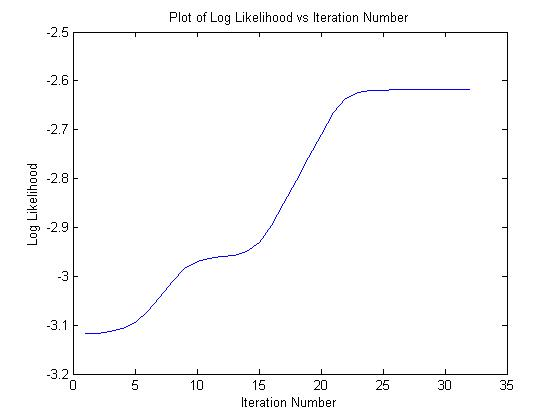
\includegraphics[height=3.25in]{dataset2_EMlogLikelihoodPlot.jpg}
\caption{The likelihood plot for dataset2, K=3, using initialization method 1}
\end{figure}

\subsection{Comments on k-Means and EM Results}

With dataset2, there was a substantial difference between the two methods. The EM algorithm seemed to capture the clusters much better than k-Means. This is likely due to the fact that two of the Gaussians used to generate the data had an overlapping mean. Since k-Means just clusters them into groups, it would struggle to group those two sets. However, EM is specifically fitting the data to Gaussians. It was thus much better to use the EM algorithm to cluster this data set. For the initialization method, assigning random member weights proved to be the best one when I compared the methods. It is to be expected that there would not be much of a difference between random member weights and using k-Means when initializing the data due to the fact that k-Means did not give us representative groups in the first place. 

\subsection{Comments on BIC test results}

\begin{table}[H]
  \centering
  \begin{tabular}{|c|c|c|}
    \hline
    \multicolumn{3}{|c|}{Dataset 2} \\\hline
    K & log likelihood & BIC value \\\hline
    1 & -4676.77 & -4698.72 \\
		2 & -4449.92 & -4493.80 \\
		3 & -3993.20 & -3993.20 \\
		4 & -3922.58 & -4010.34 \\
    5 & -3921.62 & -4031.31 \\\hline
  \end{tabular}
\end{table}

For dataset2 as with the other data sets, the log likelihood increases when we increase K, the number of clusters. When computing the BIC value, we find that it is maximized at K=3. This is what we want since the data was generated from 3 Gaussians so we wanted the best result to occur when we put the data into 3 clusters. 

\section{Plots for Dataset3}

\begin{figure}[H]
\centering
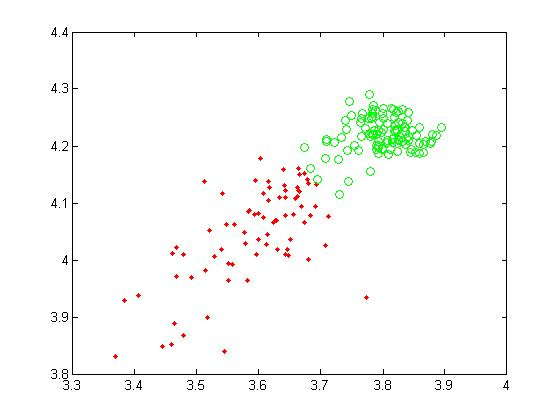
\includegraphics[height=3.25in]{dataset3_kMeansPlot.jpg}
\caption{The k-Means plot for dataset3, K=2}
\end{figure}

\begin{figure}[H]
\centering
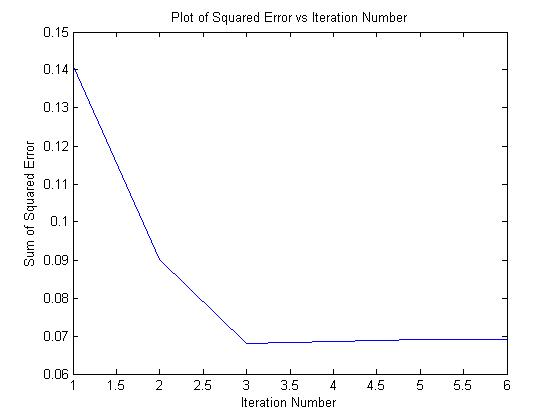
\includegraphics[height=3.25in]{dataset3_kMeans_squaredErrorPlot.jpg}
\caption{The Sum of Squared Error plot for dataset3, K=2}
\end{figure}

\begin{figure}[H]
\centering
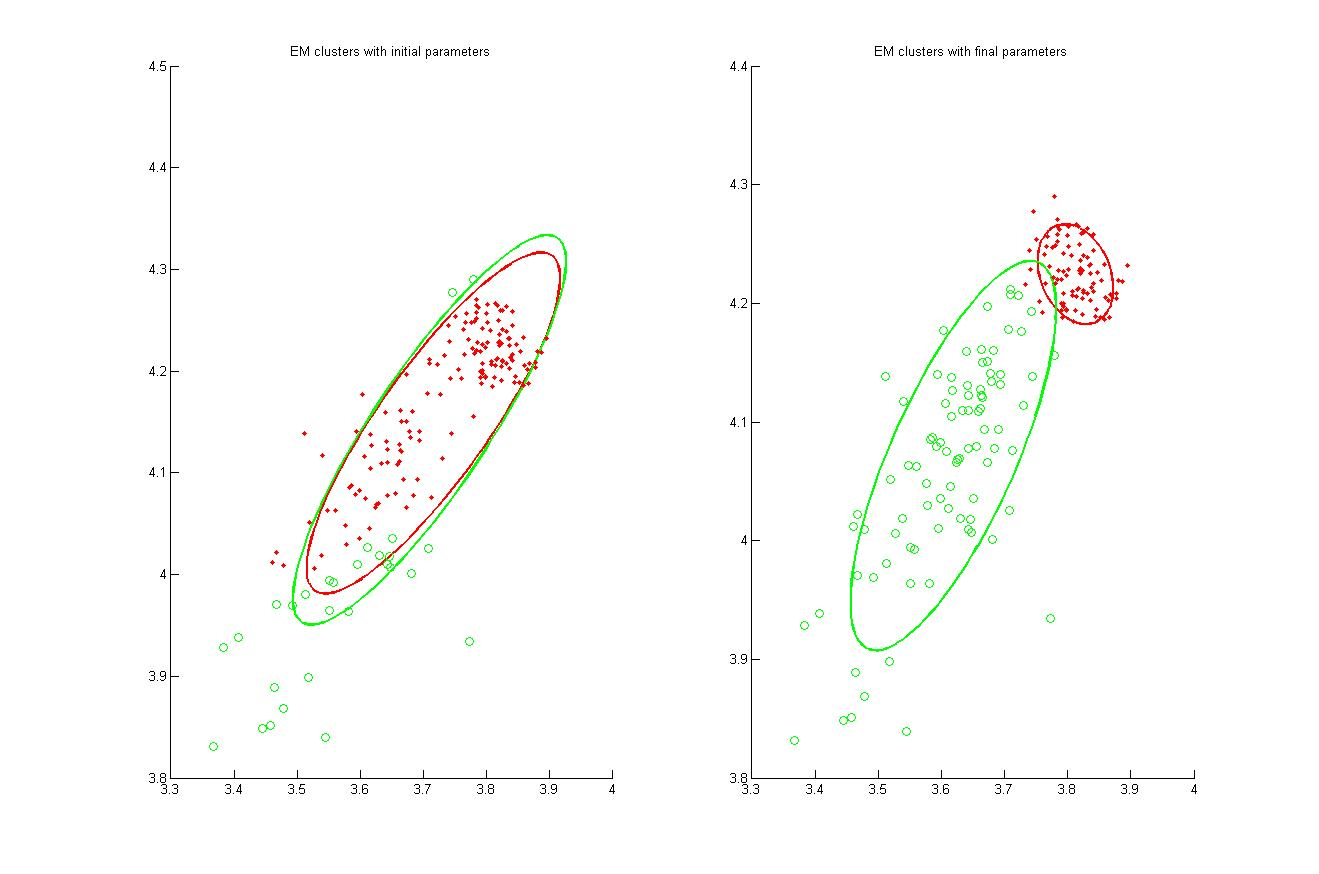
\includegraphics[height=3.25in]{dataset3_EMclusterPlots.jpg}
\caption{The EM cluster plots for dataset3, K=2, using initialization method 3}
\end{figure}

\begin{figure}[H]
\centering
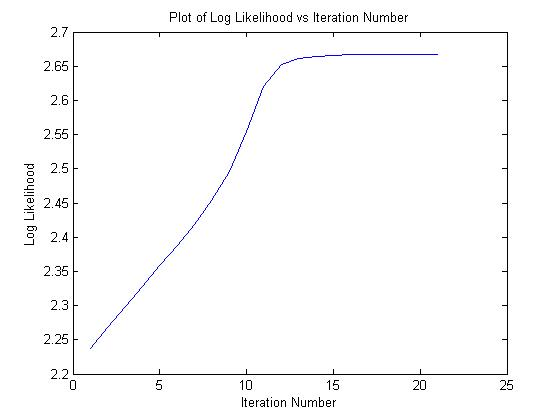
\includegraphics[height=3.25in]{dataset3_EMlogLikelihoodPlot.jpg}
\caption{The likelihood plot for dataset3, K=2, using initialization method 3}
\end{figure}

\subsection{Comments on k-Means and EM Results}

For dataset3, we are trying to take real world patient data and cluster the patients into two groups. Both methods perform very well in this case likely due to the fact that there are no two overlapping cluster centers. I calculated the accuracy of the cluster results and found that the EM algorithm has an accuracy of 96.7\%. The k-Means algorithm produced an accuracy of 96.15\%. Thus, EM did end up performing slightly better but not by much at clustering our data. This could be because in general the two groups of patients possibly have a normal distribution for those numbers so if we got more data, then EM would possibly perform even better. When I went to calculate the best initialization method for the EM run, k-Means proved to be the best one. This is to be expected because it performed very well at clustering the data in the beginning. 

\subsection{Comments on BIC test results}

\begin{table}[H]
  \centering
  \begin{tabular}{|c|c|c|}
    \hline
    \multicolumn{3}{|c|}{Dataset 3} \\\hline
    K & log likelihood & BIC value \\\hline
    1 & 402.79 & 387.17 \\
		2 & 485.35 & 454.13 \\
		3 & 494.04 & 447.20 \\
		4 & 503.97 & 441.52 \\
    5 & 507.75 & 429.69 \\\hline
  \end{tabular}
\end{table}

For dataset3, as with the other data sets, the likelihood increases as K increases. However, the BIC value is maximized at K=2. This is exactly what we want since we want to cluster patients into two groups. 

\end{document}
